%!TEX root = origin_elements_lecture_notes.tex

\chapter{Classical Novae}\label{ch:novae}

In 1572, Tycho Brahe observed a new star and described the observation in his book ``De nova stella'' (``Concerning the new star''). While the event Brahe observed was in fact a \acf{sn}, other types of new stars, generally referred to as novae, can show up in the night sky as well. These are generally not new stars, but rather the explosive final breaths of a fairly old star.

\section{Observations}

Classical novae are stellar explosions that, similar to \acp{sn}, exhibit a sudden rise in their luminosity reaching peak values of up to $10^5\,L_\odot$. Similar to \ac{snia}, these explosions take place in binary star systems that consist of a \acf{wd} and a low-mass companion star that is typically on the main sequence. While novae are among the most frequent types of thermonuclear explosions in the galaxy with rates of around 30\,a$^{-1}$ per galaxy, they release about six orders of magnitude less energy than \acp{sn}.
\begin{figure}[tb]
    \centering
    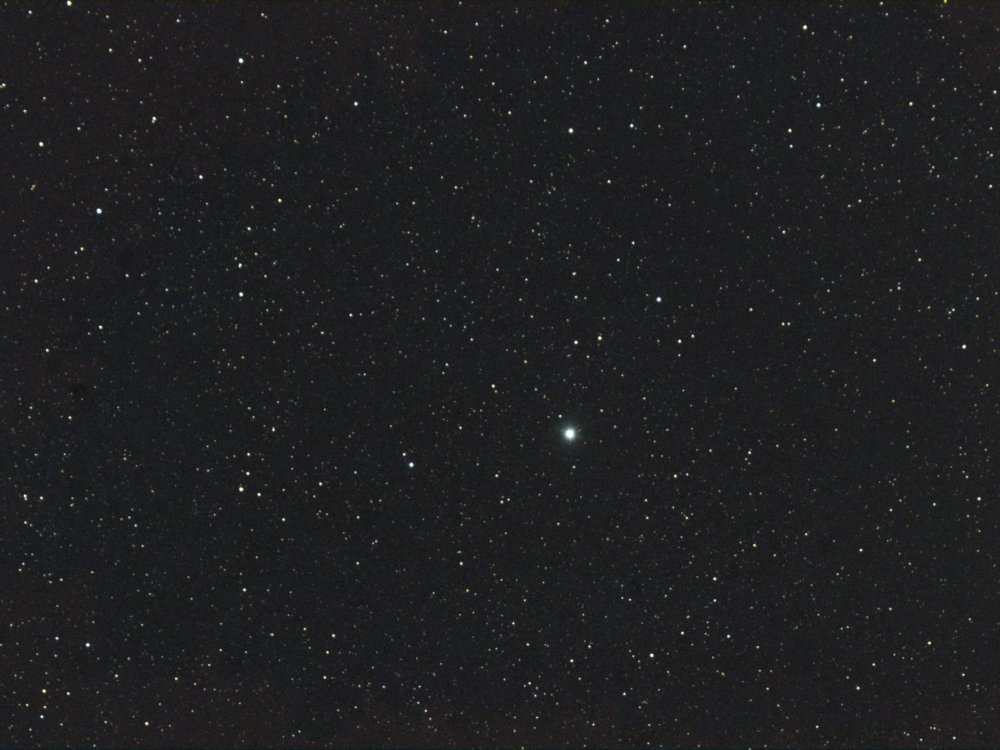
\includegraphics[width=0.8\textwidth]{graphics/novae/nova_v1369}
    \caption{Nova V1369 Centauri, which was visible in the Soutern Hemisphere in 2013. The star became around $10^4$ times brighter than usual. Image Credit: \href{https://www.nasa.gov/watchtheskies/new-nova-star-australia.html}{NASA/MSFC/ESSSA/Aaron Kingery}.}
    \label{fig:novae:nova_v1369}
\end{figure}
An example of such a classical nova event is shown in Figure~\ref{fig:novae:nova_v1369}. This image shows nova V1369 Centauri, which took place in 2013 and was visible from the Southern Hemisphere. During its peak luminosity, the star was around $10^4$ times brighter than usual. 

The peak brightness of novae fades over weeks and months, depending on the exact conditions that led to the explosion in the first place. Furthermore, a specific type of recurrent novae have been discovered. These stellar explosions repeat regularly with intervals of 10 to 100\,a. 

The peak brightness of classical novae fades fast since these events are copious dust producers. During the thermonuclear runaway, mass is effectively ejected from the star into interstellar space, where it condenses into dust. This dust then blocks the visible light. Dust production has been confirmed by observations. While the visible brightness of a classical novae fades fast, the total brightness including infrared radiation stays high for much longer, further implying the production of dust. This dust is recycled back into the galaxy, making classical novae significant contributors to \ac{gce}. Furthermore, since the maximum temperature that can be reached during the thermonuclear runaway is limited, as we will see below, only a small range of isotopes can potentially be produced and thus, only a small reaction rate network must be included to calculate nova nucleosynthesis. The fact that such a limited network produces observable dust makes classical novae an ideal test bed for nucleosynthesis calculations.


\section{Evolution of a Classical Nova}

Similar to \acf{snia}, classical novae occur in binary star systems in which a \ac{wd} is accreting mass from a companion star. This scenario has been shown in Figure~\ref{fig:massive_stars:sn_ia_artistic} and can be pictured similarly. In order for mass transfer from one star to the other to occur, the two stars have to be close to each other such that mass transfer via the Roche Lobe overflow is possible. For this to occur, the outer atmosphere of the companion star must be inside the gravitational potential of the \ac{wd}, leading to accretion of hydrogen onto the \ac{wd}. 


\subsection{Overview}

\begin{figure}[tb]
    \centering
    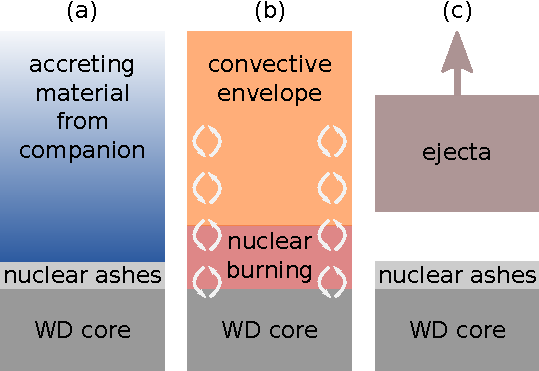
\includegraphics[width=0.6\textwidth]{graphics/novae/nova_schematic}
    \caption{Schematic of a nova explosion in three steps. See text for details. After \citet{iliadis18}.}
    \label{fig:novae:schematic_of_thermonuclear_runaway}
\end{figure}
Figure~\ref{fig:novae:schematic_of_thermonuclear_runaway} shows a schematic of the evolution of a thermonuclear runaway in a classical nova explosion. At the center is the \ac{wd}, labeled ``\ac{wd} core''. On top of the \ac{wd} lay nuclear ashes from previous nova explosions. These are leftovers that did not get ejected.

Over long periods of time (panel a), the \ac{wd} accretes hydrogen from its main sequence companion star due to Roche Lobe overflow. Therefore, nuclear fuel accumulates slowly (blue part of panel a). The bottom of this layer is continuously compressed due to surface gravity, becomes degenerate, and heats up. As the bottom heats up, hydrogen burning sets in; first via the \ac{pp-chain}, later via the CNO-cycle. Since the matter is electron degenerate, the increase in temperature does not lead to an increase in the pressure since these two quantities are independent (see also the discussion of electron degenerate matter on page~\pageref{box:sun:electron_degenerate_matter}). These conditions lay the groundwork for a thermonuclear runaway. Heating in the nuclear burning layers creates instabilities in the star which induces convection (panel b). Convection (1) mix freshly nucleosynthesized material throughout the envelope and (2) dredge up material from the \ac{wd} core, mixing it into the envelope. Since at this point hydrogen burning mainly takes place via the CNO-cycle, unstable nuclei such as \ex{13}N, \ex{14}O, \ex{15}O, and \ex{17}F are mixed into the whole envelope (see also Figure~\ref{fig:sun:cno_cycle} for a schematic of the CNO cycle). These nuclides deposit energy into the outer, cooler envelope as they decay. Part of this energy is transformed into kinetic energy, which supports the expansion of the envelope. Once enough radiation pressure is achieved in the nuclear burning zone, mass ejection of part of the star will take place (panel c). This effectively stops the nuclear burning by expansion and thus cooling of the envelope. Only some nuclear ashes are left behind. 

Once matter is ejected, accretion from the companion star can start again and the \ac{wd} starts building up another hydrogen envelope on top of the nuclear ashes. When enough matter is accreted, the thermonuclear runaway will occur once more. This makes classical novae recurring events.
\begin{table}[tb]
\infobox{Roche Lobe}{The Roche Lobe of, e.g., a binary star system, is the gravitational equipotential line of the system. The outline of the lobe is tear-drop shaped with a a well defined point in between the two bodies. This point is also known as the Lagrangian 
L$_1$ point. An object that is placed in L$_1$ is by definition at a graviationally neutral position between the two objects. See also \href{https://en.wikipedia.org/wiki/Roche_lobe}{Wikipedia} for more detail.

In chapter~\ref{ch:solar_system_abundances} we have discussed the Genesis mission. This spacecraft was placed at the L$_1$ point in between the Earth and the Sun for more than a year in order to collect solar wind. Such a ``parking'' position is of course ideal in order to collect particles from the Sun since it is never in the Earth's shadow.}
\end{table}

\subsection{Mass Ejection}

In order to account for mass ejection, a so-called proper pressure of $P_\star \geq 10^{19}$\,Pa is required \citep{jose12}. This pressure depends on the mass of the \ac{wd} ($M_\mathrm{WD}$), its radius ($R_\mathrm{WD}$) and the mass of the accreted matter ($M_\mathrm{accr}$) as
\begin{equation}
    P_\star = \frac{GM_\mathrm{WD}}{4\pi R_\mathrm{WD}^4} M_\mathrm{accr}.
\end{equation}
Here, $G$ is the gravitational constant. This shows that shorter timescales for nova explosions are expected for heavier \acp{wd}. 

Once the mass is ejected, it rapidly cools down and starts forming dust. This dust formation then moves the main luminosity of the classical nova event from visible wavelengths to infrared while the peak luminosity stays the same for some time. The ejection of $\beta$-unstable nuclei that form in the CNO cycle yields a very large production of \ex{13}C from \ex{13}N decay, \ex{15}N from \ex{15}O decay, and \ex{17}O from \ex{17}F decay. Classical novae are in fact the main source for the production of these nuclei.


\subsection{Open questions}\label{sec:novae:open_questions}

One dimensional nova models can successfully reproduce many of the observable parameters, however, two major open questions remain in order to better understand classical novae. First, it is unclear how exactly the convective region (panel b in Figure~\ref{fig:novae:schematic_of_thermonuclear_runaway}) develops. Multidimensional classical nova simulations, see, e.g., reviews by \citet{jose12} and \citet{starrfield16}, are being employed to better answer these questions. However, such simulations still cannot fully explain all observables, e.g., asymmetric dust creation in nova ejecta and stardust grain compositions.

Second it is also unclear how and when material from the \ac{wd} are mixed into the accreted nuclear fuel. Classical novae are in fact classified by the type of matter they contain in their spectra. Depending on the \ac{wd} that is at the center of these events, the ejected matter contains either CO or ONe, thus making it a CO nova or an ONe nova, respectively. The ejecta classifying the nova type is the material originally dredged up from the \ac{wd}, which furthermore also supplies seeds for charged particle reactions and thus, defines the final composition of the nucleosynthesized material. Understanding this dredge up is therefore crucial in order to adequately model nucleosynthesis in classical novae.



\section{Nova Nucleosynthesis}

Classical novae are ideal test beds for nucleosynthesis calculations. The temperatures reach high enough such that the CNO and the hot-CNO cycle are effectively activated and charged particle reactions can take place. Nucleosynthesis tops out at calcium due to the limited peak temperatures that can be achieved in these stellar explosions. This peak temperature is limited since the ejection of material effectively stops the nucleosynthesis due to envelope expansion and cooling.
\begin{figure}[tb]
    \centering
    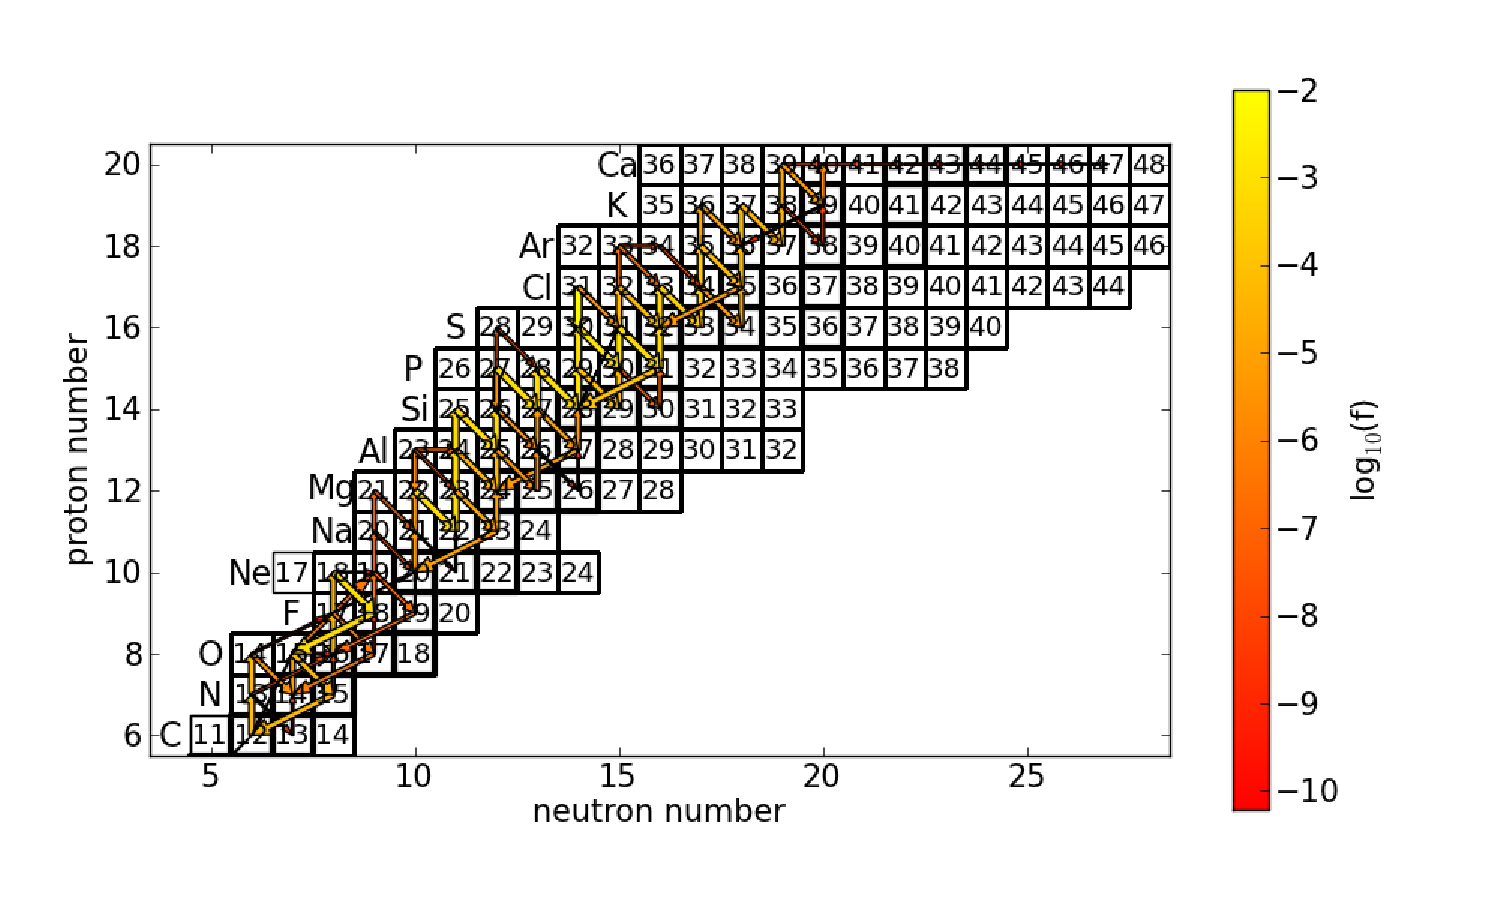
\includegraphics[width=0.8\textwidth]{graphics/novae/nova_reac_net}
    \caption{The nova reaction rate network of 147 isotopes. Figure taken from \citet{denissenkov14}.}
    \label{fig:novae_reaction_rate_network_denissenkov}
\end{figure}
Figure~\ref{fig:novae_reaction_rate_network_denissenkov} shows the reaction rate network used by \citet{denissenkov14} in their nova simulations. The width and colors of the arrows correspond to the flux strength in the simulation of an ONe nova from the start until it reaches a peak temperature of $T_8 \approx 4$.

Figure~\ref{fig:novae_reaction_rate_network_denissenkov} clearly shows that all reactions take place close to the valley of stability. The associated reaction rates are therefore directly accessible to nuclear physics experiments and have, for the most part, been measured. This makes the stellar evolution and mixing prescription the major uncertainty for classical nova nucleosynthesis calculations, allowing to better study the exact nature of the open questions discussed in Section~\ref{sec:novae:open_questions}.


\section{Stardust from Novae}

As shown in Figure~\ref{fig:stardust:classification_c_n_si_data}, several putative novae grains have been found over the years. These grains show, as expected, large enrichments in \ex{13}C and \ex{15}N. However, in order to explain the multi-isotopic composition of many of the putative nova grains, mixing between freshly nucleosynthesized nova material with solar-like material is required since the isotopic signal the grains carry does not agree directly with the nucleosynthesis calculations. The nova isotopic composition for most grains has to be mixed or diluted and the overall composition of stardust grains of potential nova origin are usually composed of $\geq 90$\% solar composition material. The origin and mechanism for this mixing has been extensively debated in the literature over the years, so far without clear success.


\subsection{Monte Carlo Simulations}

Recently, \citet{iliadis18} used \ac{mc} simulations of classical nova explosions to identify 18 presolar grains with measured isotopic signatures that agree with a CO nova origin. For these grains, no dilution of the nova ejecta has to be assumed in order to explain their isotopic composition. 

In order to perform \ac{mc} calculations of nucleosynthesis in classical novae, \citet{iliadis18} used so-called one zone models for stellar evolution. In these models, all nucleosynthesis happens in one area, for which the temperature and density can be parameterized based on the peak values as
\begin{align}
    T(t) &= T_\mathrm{peak} \exp{\left(\frac{-t}{\tau_T}\right)} \\
    \rho(t) &= \rho_\mathrm{peak} \exp{\left(\frac{-t}{\tau_\rho}\right)}.
\end{align}
Here, $t \geq 0$ is the time since peak temperature $T_\mathrm{peak}$ and peak density $\rho_\mathrm{peak}$. The variables $\tau_T$ and $\tau_\rho$ are the times at which the temperature and density, respectively, have fallen to $1/e$ of their peak values. Thus, the peak temperature and density in the one zone model are expected to decay analogously to a radioactive decay with $\tau$ as the ``lifetime'' of the state. While these nova models are heavily simplified, \citet{iliadis18} showed that they can in fact be applied to predict isotope ratios of nucleosynthesis events that is taking place in novae. Nucleosynthesis calculations in these models included a reaction rate network including a total of 213 nuclides and 2373 reaction rates. 

\begin{figure}[tb]
    \centering
    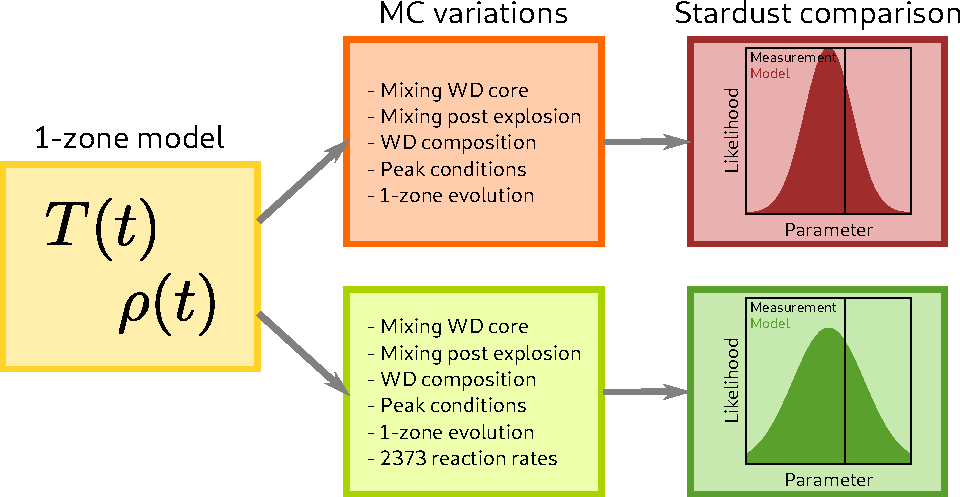
\includegraphics[width=0.8\textwidth]{graphics/novae/mc_model_iliadis_schematic}
    \caption{Simplified flowchart of the \ac{mc} model used by \citet{iliadis18}.}
    \label{fig:novae:mc_model_iliadis_flowchart}
\end{figure}
Figure~\ref{fig:novae:mc_model_iliadis_flowchart} shows a simplified flowchart of the \ac{mc} model used by \citet{iliadis18}. Two sets of \ac{mc} variations are run with starting from their one zone model, shown in the figure as the top (simplified) and bottom (full) path. The simplified \ac{mc} variations only consider the main uncertainties of the evolution and vary all of these parameters within reasonable ranges. The key parameters here are the peak temperature and density and the associated $\tau$ values for the 1-zone evolution, the \ac{wd} composition, the mixing fraction of the \ac{wd} core with the nuclear burning region, and the post-explosion mixing fraction with solar-like material. Thus, the simplified model only varies the stellar parameters. The more complex \ac{mc} model also varies the reaction rates in addition. \citet{iliadis18} showed that these reaction rates are not the dominating factors and only slightly broaden the possible outcomes. The main factors contributing to uncertainties are the stellar evolution parameters, as shown in the top path of Figure~\ref{fig:novae:mc_model_iliadis_flowchart}. 

Using these \ac{mc} parameter variations, \citet{iliadis18} showed that the measurements of 18 stardust grains in total agree with an origin in CO novae even when no dilution with solar-like material is taken into account. Varying the parameters of the nova models themselves was enough to show that grain measurements can be explained by classical novae explosions and that the nucleosynthetic output is not as well constrained as previously thought. These results are of great importance since they show that the details of classical novae explosions are poorly understood. Future, 3D hydrodynamics simulations will be required to elaborate on these results and further determine the range of the free parameters used in the \ac{mc} model. The one zone models hereby can be used to give a first hint on which parameters are indeed highly critical. Clearly, the reaction rate network and involved isotopes are at this point well enough understood such that stardust analyzes of novae grains can be used to directly constrain the stellar models themselves.


\subsection{Mixed Messages from a Nova Outburst}

One of the stardust grains that was analyzed by \citet{iliadis18} for a potential nova origin was grain LAP-149, a $1\,\mu$m croissant-shaped grain found in situ in the primitive carbonaceous chondrite LaPaz Icefield 031117 and originally reported on by \citet{haenecour16}. \citet{iliadis18} concluded that this grain is unlikely of nova origin due to the measured oxygen isotopic composition, which does not agree with nova model outputs. Subsequently, the grain was further analyzed by \citet{haenecour19}. These authors stated that there is a general discrepancy between nova grains and oxygen nucleosynthesis calculations of novae, arguing that LAP-149 indeed originated from a novaj. \citet{haenecour19} furthermore discovered that the graphite grain LAP-149 contains a $\sim100$\,nm oxide inclusion. Graphite cannot condense in oxygen-rich environments. On the other hand, oxygen-rich conditions are required for oxide condensation. Thus, these grains must have formed in different zones of the classical nova ejecta and subsequently been mixed.

\begin{figure}[tb]
    \centering
    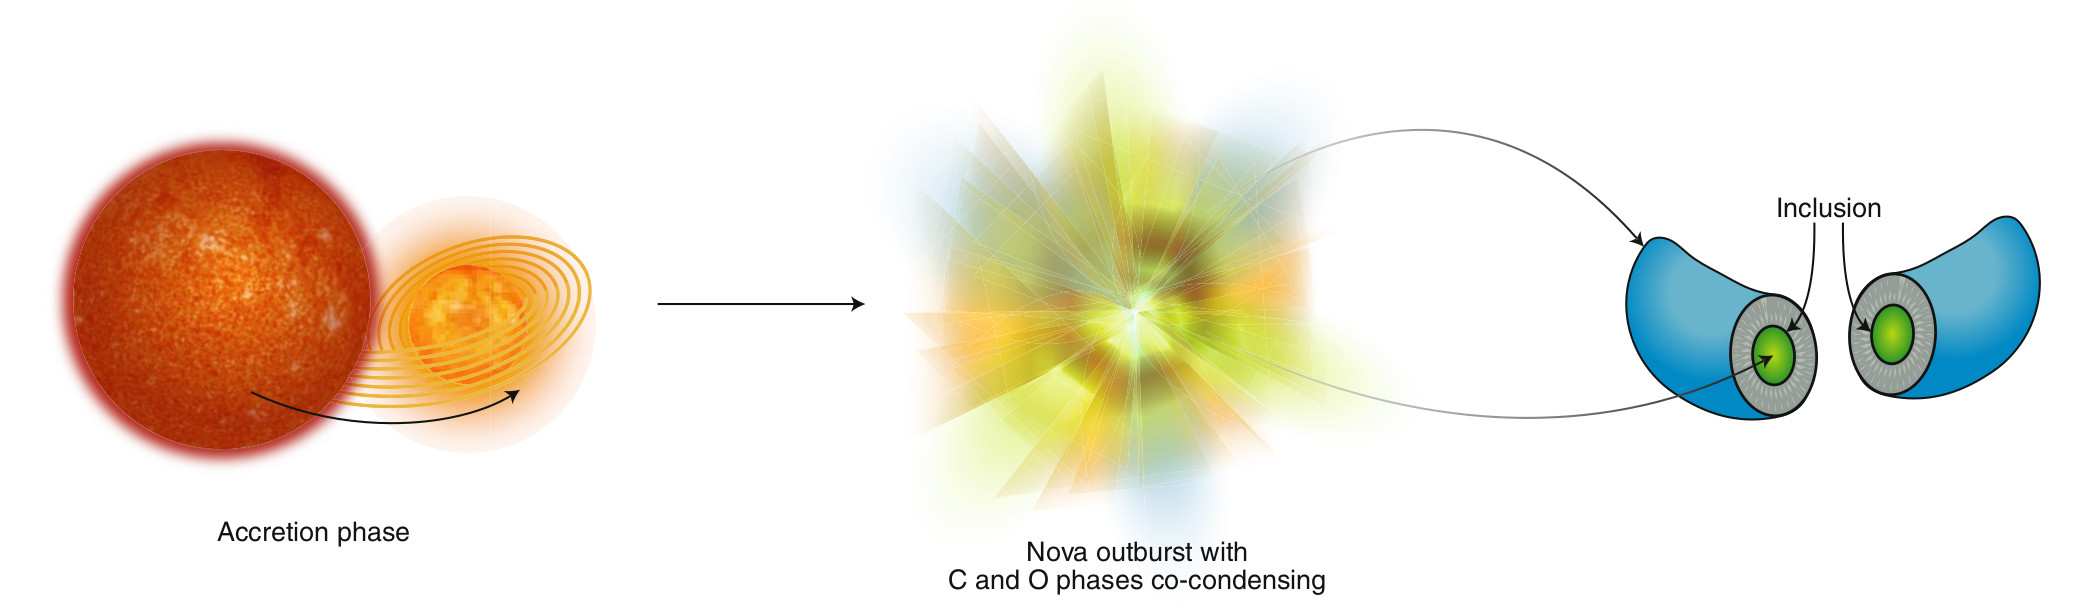
\includegraphics[width=\textwidth]{graphics/novae/nova_schematic_nature_astro}
    \caption{Schematic of the classical nova accretion, subsequent explosion, and mixing required in order to explain the composition of nova grain LAP-149. From \citet{trappitsch19}.}
    \label{fig:novae:mixing_schematic_nova_nature_astronomy}
\end{figure}
Figure~\ref{fig:novae:mixing_schematic_nova_nature_astronomy} shows an impression of the scenario that could have led to the formation of grain LAP-149 \citep{trappitsch19}. As discussed previously, the \ac{wd} accretes matter from a companion star until the thermonuclear runaway sets in and ultimately leads to ejection of nova material. Here, the figure schematically shows the scenario in which the oxide grain first condensed in an oxygen-rich zone, was then transported to a carbon-rich area in which graphite then condensed around the oxygen subgrain. Both, temporal or spatial heterogeneity could explain the observed grain. Asymmetric explosions have furthermore been observed for classical novae and it has been shown that carbonaceous and silicate dust co-condenses in novae outflows within 50 to 100 days after the explosion. Presolar grain LAP-149 shows the first direct laboratory evidence for this co-condensation. Future classical nova models are required in order to explain how this heterogeneity can take place and how mixing might indeed yield stardust grains such as the one found by \citet{haenecour19}.


\section{Reading}

Manuscripts that further elaborate on the discussed materials have already been mentioned in the notes above. The curious reader might want to start out with reading \citet{jose12} for a better overview of classical nova and, especially, of multidimensional hydrodynamics simulations. Furthermore, the work by \citet{iliadis18} discusses well the compoarison of stardust grains and nova models and introduces the interesting concept of \ac{mc} modeling to achieve this difficult task.